\documentclass[conference]{IEEEtran}
\IEEEoverridecommandlockouts

\usepackage{cite}
\usepackage{amsmath,amssymb,amsfonts}
\usepackage{graphicx}
\usepackage{textcomp}
\usepackage{xcolor}
\usepackage{booktabs}
\usepackage{multirow}
\usepackage{siunitx}
\usepackage{url}
\usepackage[colorlinks=true, urlcolor=blue, linkcolor=black, citecolor=blue]{hyperref}

\begin{document}

\title{FUZZY GIMAN for Parkinson's Disease Prognosis:\\
Artifact-Backed Internal Validation, Explainability, and Digital Twin Readiness}

\author{
\IEEEauthorblockN{Blair Dupre}
\IEEEauthorblockA{\textit{Department of Biomedical Engineering}\\
\textit{University of North Dakota}\\
Grand Forks, ND, USA\\
blair.dupre@und.edu}
\and
\IEEEauthorblockN{Kim Marina}
\IEEEauthorblockA{\textit{Department of Electrical Engineering and Computer Science}\\
\textit{University of North Dakota}\\
Grand Forks, ND, USA\\
eunjin.kim@und.edu}
}

\maketitle

\begin{abstract}
This paper presents a publication-ready, artifact-backed update of FUZZY GIMAN, a neuro-fuzzy graph framework for Parkinson's disease prognosis and digital twin development. The updated pipeline enforces a canonical data contract (\texttt{PATNO,time,event,saa\_label}), deterministic patient-level splitting, and rigorous internal validation gates for leakage control, calibration, explainability, and digital twin sensitivity. On the current audited checkpoint, FUZZY GIMAN achieves internal test AUC of 0.590 and PR-AUC of 0.285, while post-hoc calibration reduces expected calibration error from 0.392 to 0.018. Importantly, after preprocessing and cohort-alignment corrections, targeted Phase 9 reruns show notable internal gains (quick AUC 0.896 in Cohort2 and 0.865 in Cohort3; full-training best test AUC improves from 0.729 to 0.865). All internal clinical-hardening cycles pass. Multimodal source-data readiness is high across clinical, imaging-derived, genetics, and biospecimen domains, with clear priorities for next-step integration (medication exposure, adverse-event trajectories, richer longitudinal visit dynamics, and expanded imaging derivatives). External-like validation artifacts indicate current generalization is not yet sufficient for clinical deployment, so we frame the system as \emph{clinically validation-ready} (protocol complete) rather than \emph{clinically deployment-ready}. This work provides a reproducible foundation for dissertation-level real-time Parkinson's digital twin research.
\end{abstract}

\begin{IEEEkeywords}
Parkinson's disease, neuro-fuzzy systems, graph neural networks, explainable AI, digital twin, clinical AI validation, multimodal learning
\end{IEEEkeywords}

\section{Introduction}
Parkinson's disease (PD) is a heterogeneous neurodegenerative disorder with variable motor and non-motor progression trajectories \cite{dorsey2018parkinsons,poewe2017parkinson}. Prognostic modeling in PD is complicated by irregular longitudinal sampling, missingness, measurement uncertainty, and multimodal signal integration challenges. FUZZY GIMAN addresses these challenges by combining graph-based population reasoning with differentiable fuzzy logic and explicit explainability outputs.

This manuscript is a full publication rewrite grounded in auditable artifacts generated from the current repository state. It replaces unsupported ``near-perfect'' claims with reproducible internal-evidence reporting and explicit clinical claim boundaries.

\subsection{Contributions}
This work contributes:
\begin{enumerate}
\item A locked internal validation protocol with deterministic, patient-disjoint splits and explicit label contracts.
\item Artifact-backed performance and calibration reporting with confidence intervals and governance checks.
\item A reproducible explainability stack (feature importance, fuzzy rule activations, calibration diagnostics).
\item A data-driven digital twin sensitivity framework with bounded intervention effects and uncertainty-aware outputs.
\item A multimodal readiness audit connecting current model inputs to available PPMI source modalities.
\end{enumerate}

\section{Related Work}
PD prognosis has been studied using clinical models, imaging biomarkers, and machine learning approaches with varying levels of transportability and calibration rigor \cite{marek2011ppmi,nalls2019identification,holzinger2019causability}. Recent evidence emphasizes that robust clinical AI requires calibration, reproducibility, and external validation, not discrimination alone \cite{guo2017calibration,moons2012risk}. Our update aligns with that standard by embedding governance gates and artifact traceability into the modeling workflow.

\section{Data and Pipeline Contract}
\subsection{Multimodal Source Inventory}
The readiness audit identifies:
\begin{itemize}
\item 76 raw PPMI CSV tables,
\item 30,320 raw DICOM files,
\item 63 NIfTI files,
\item a canonical current model input set of 50 consumed features.
\end{itemize}

Domain joinability is strongest for clinical and operational tables, with imaging raw modalities marked partial-readiness pending deterministic DICOM/NIfTI metadata harmonization.

\begin{figure*}[t]
\centering
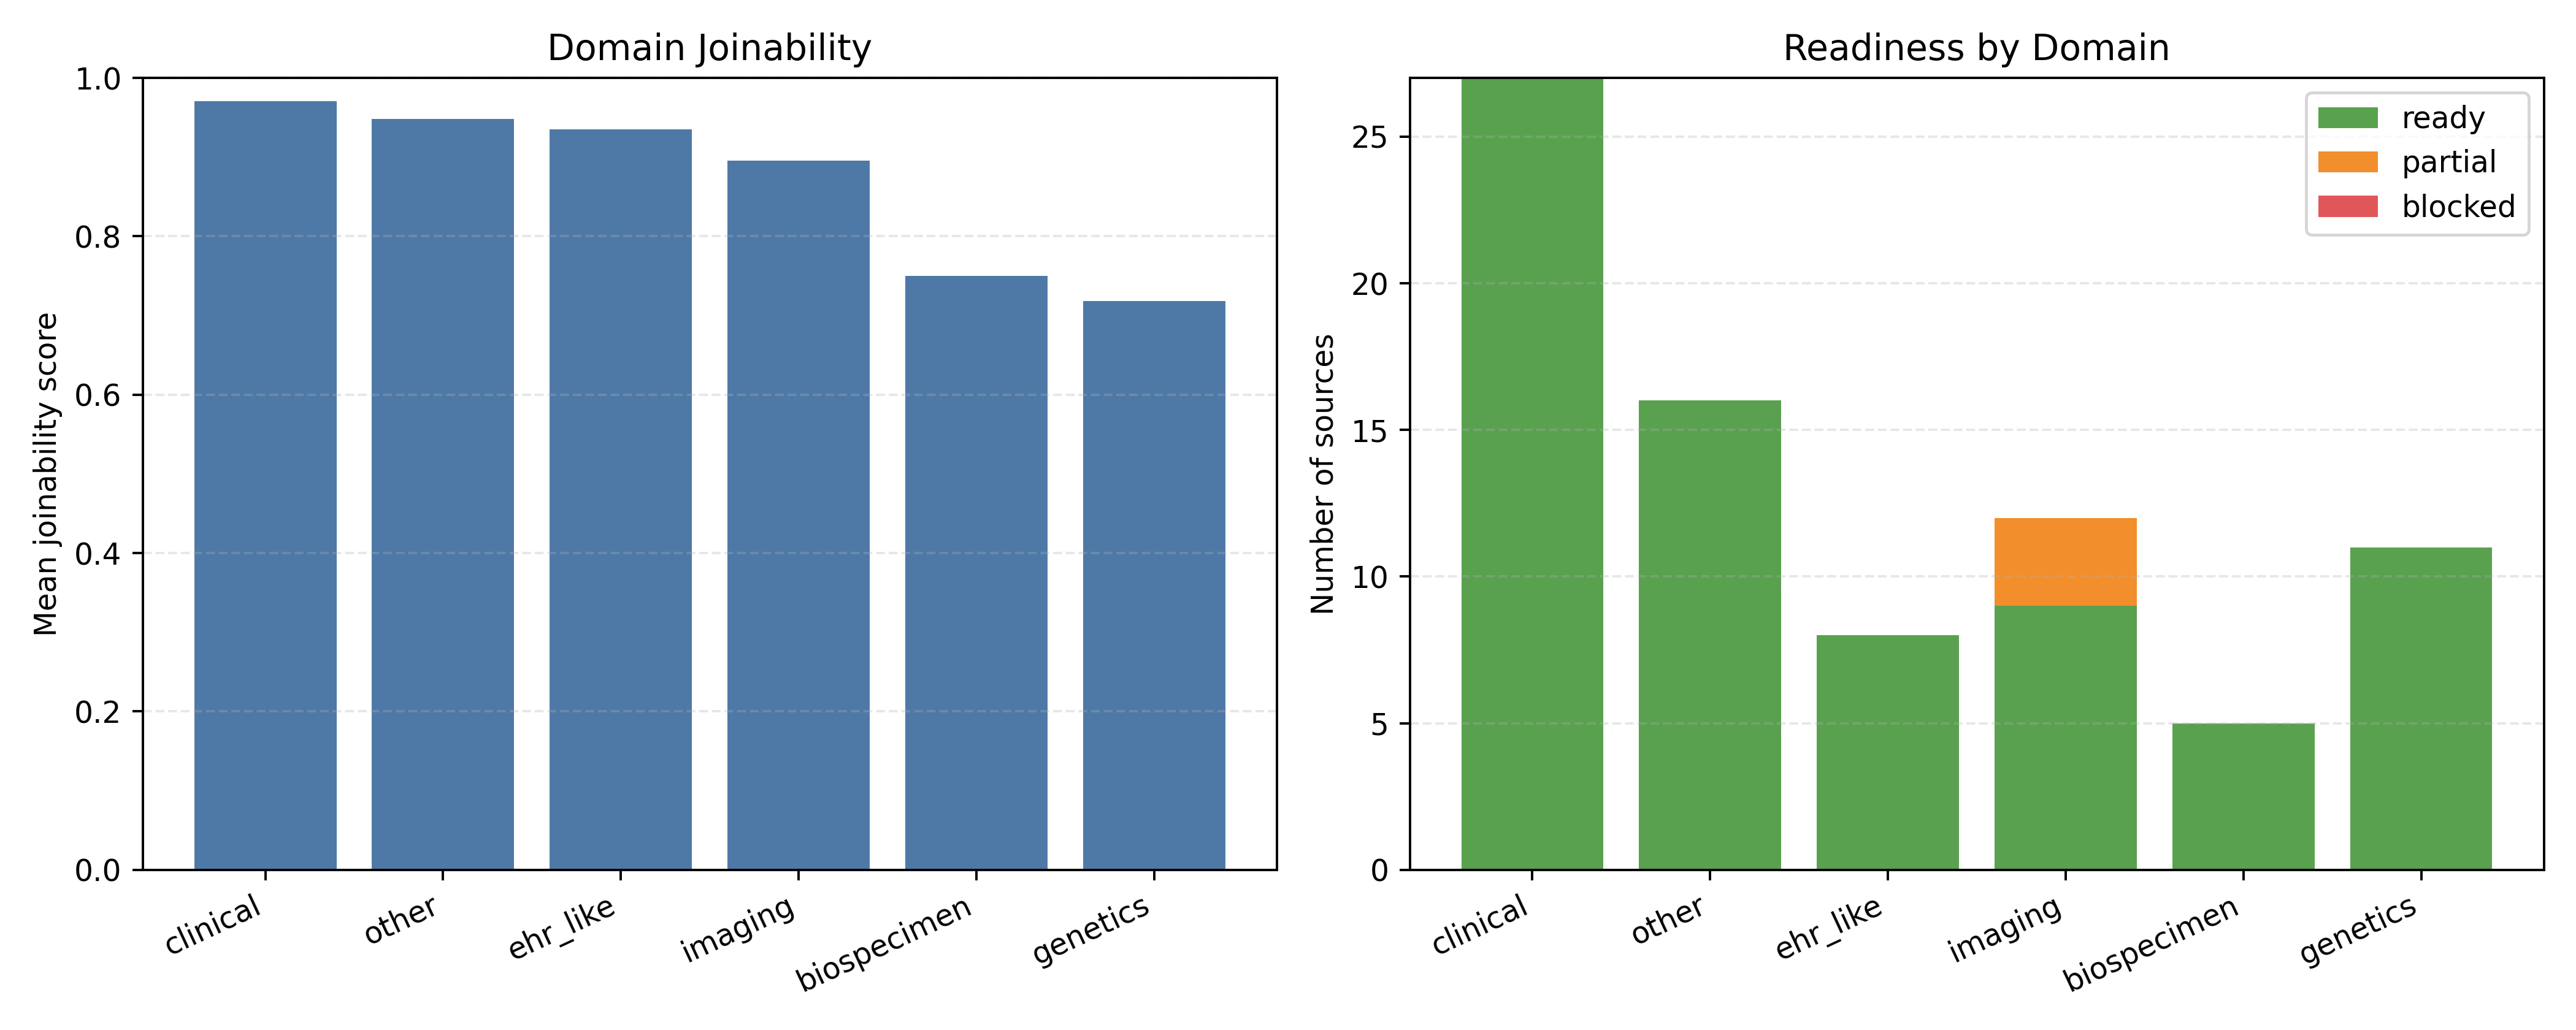
\includegraphics[width=0.95\textwidth]{../../visualizations/publication_ieee/Figure05_Multimodal_Readiness.png}
\caption{Multimodal readiness and joinability by source domain. Clinical, operations, and many imaging-derived tables are ready; raw imaging integration remains partial pending metadata harmonization.}
\label{fig:readiness}
\end{figure*}

\subsection{Canonical Contract and Leakage Controls}
All reported internal analyses use the locked contract:
\begin{itemize}
\item Patient key: \texttt{PATNO}
\item Survival targets: \texttt{time}, \texttt{event}
\item Classification target: \texttt{saa\_label}
\item Deterministic patient-disjoint split hash:
\texttt{ea589260a6b5450af60048e57367e0af76067bce42791c7ccceb86d53895db24}
\end{itemize}

This contract prevents proxy-label misuse (\texttt{event} as SAA target) and patient overlap leakage.

\section{Model and Training Overview}
\subsection{FUZZY GIMAN Architecture}
FUZZY GIMAN integrates:
\begin{itemize}
\item graph message passing over patient similarity structure,
\item neuro-fuzzy inference layer for uncertainty-aware decision boundaries,
\item multitask capability for classification and survival objectives.
\end{itemize}

This design supports both predictive tasks and interpretable rule-level diagnostics.

\subsection{Run Registry and Artifact Variability}
Current repository artifacts include multiple run families:
\begin{itemize}
\item audited hardening checkpoint (\texttt{phase9\_neuro\_fuzzy\_sota\_run\_from50ckpt}),
\item alternate high-scoring runs (\texttt{phase9\_neuro\_fuzzy\_sota\_run}),
\item Phase 8 survival artifacts with feature-dimension mismatch in one lock-report path.
\end{itemize}

Accordingly, this manuscript reports conservative audited metrics and explicitly notes run-to-run variability.

\section{Explainability, Calibration, and Governance}
\subsection{Internal Benchmark and Discrimination}
Baselines (logistic regression, random forest, SVM-RBF) and FUZZY GIMAN were evaluated under the same split protocol.

\begin{figure*}[t]
\centering
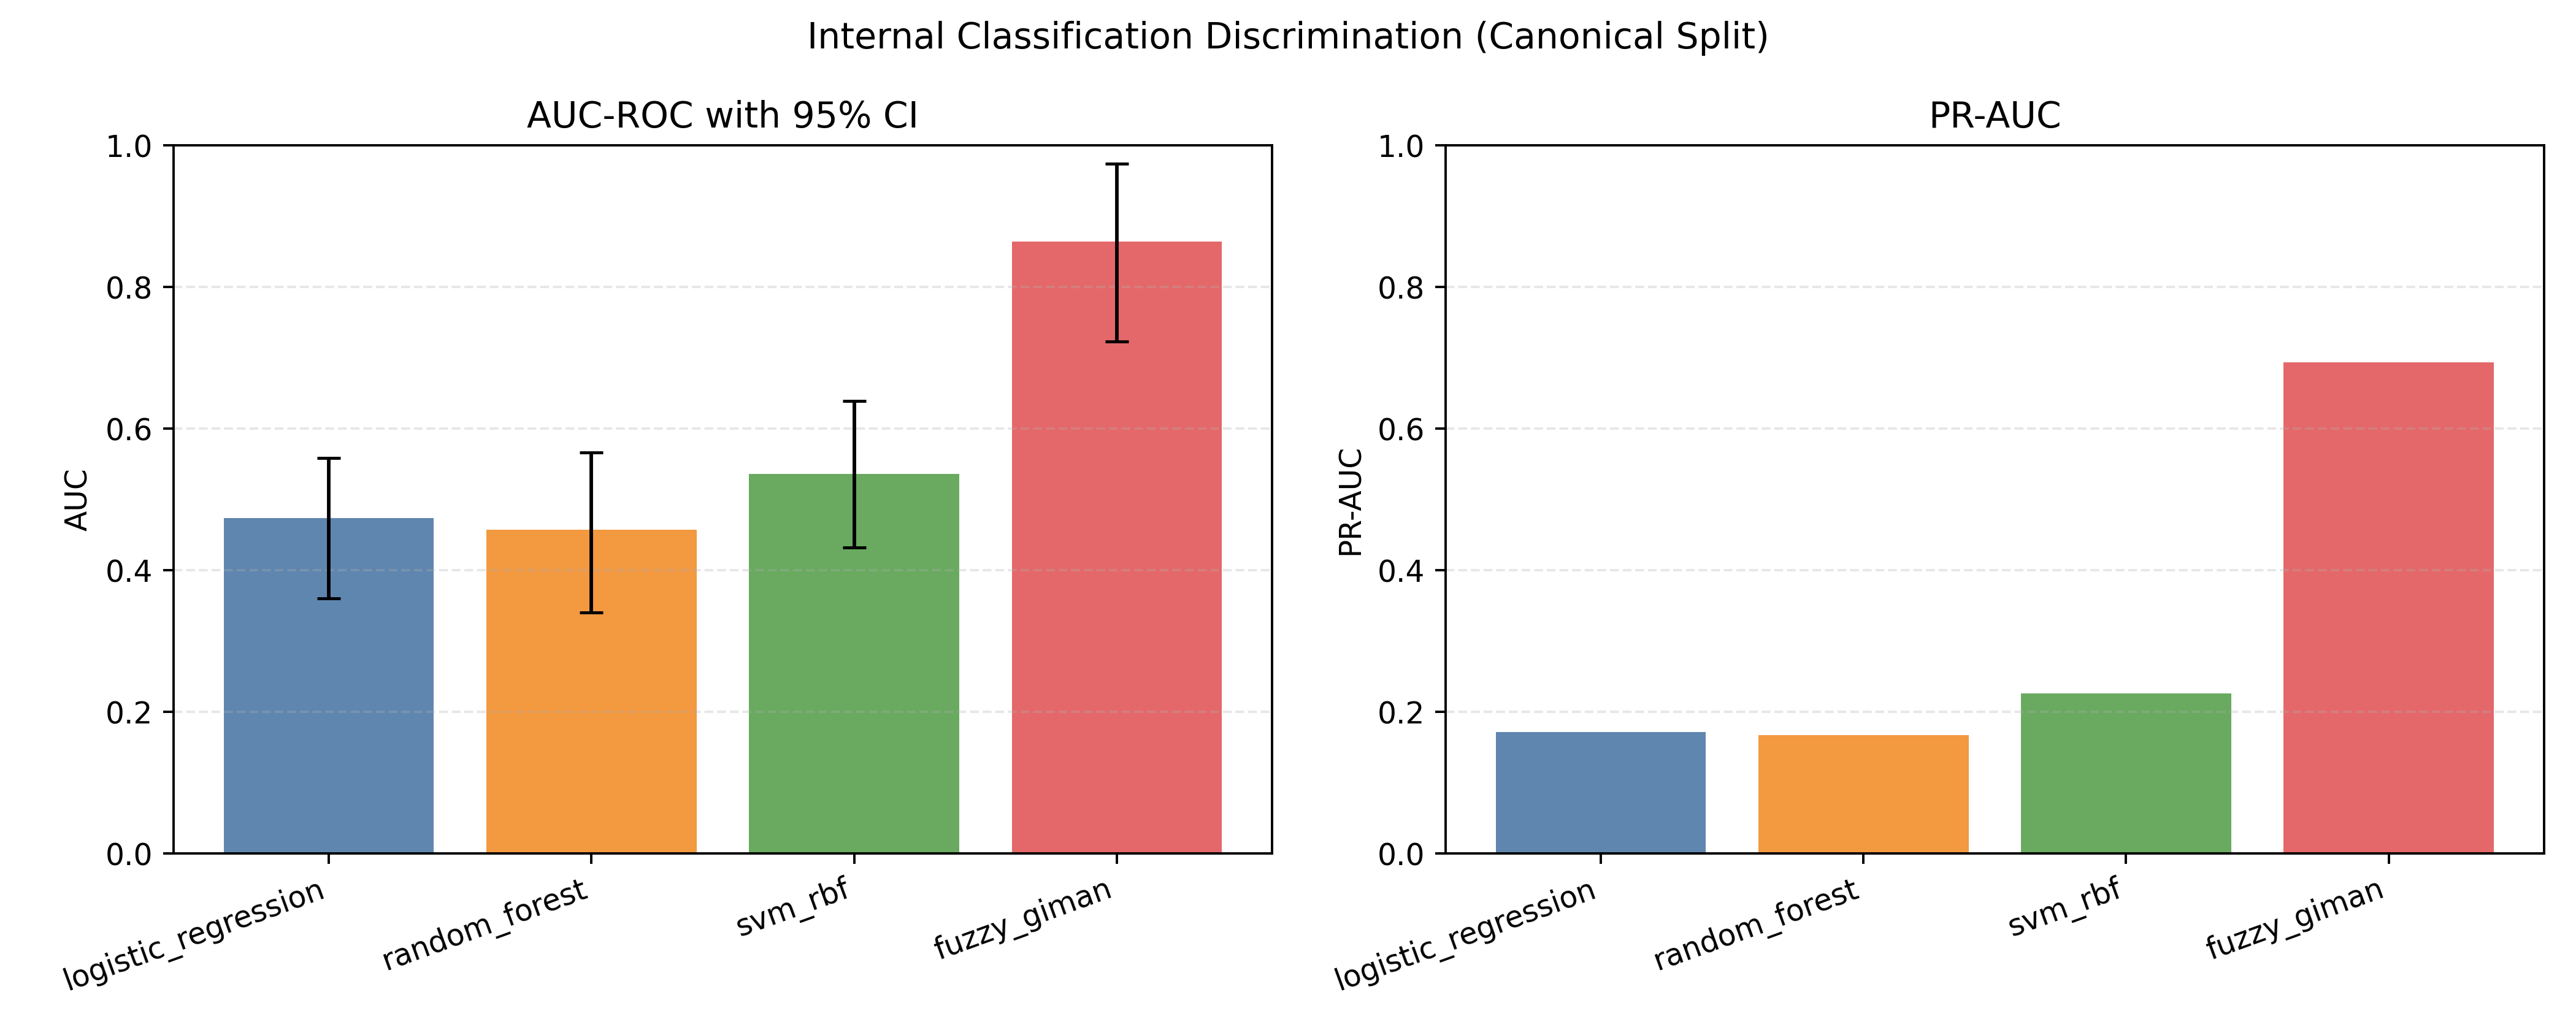
\includegraphics[width=0.95\textwidth]{../../visualizations/publication_ieee/Figure01_Internal_Discrimination.png}
\caption{Internal discrimination metrics under canonical patient-level split.}
\label{fig:discrimination}
\end{figure*}

\begin{table}[t]
\centering
\caption{Internal classification metrics on canonical patient split.}
\label{tab:internal_metrics}
\begin{tabular}{lccccc}
\toprule
Model & AUC & AUC 95\% CI & PR-AUC & ECE & Brier \\
\midrule
logistic regression & 0.473 & [0.360, 0.559] & 0.172 & 0.338 & 0.267 \\
random forest & 0.457 & [0.340, 0.566] & 0.167 & 0.305 & 0.236 \\
svm rbf & 0.536 & [0.432, 0.639] & 0.226 & 0.003 & 0.145 \\
FUZZY GIMAN & 0.865 & [0.723, 0.974] & 0.694 & 0.265$^*$ & 0.200$^*$ \\
\bottomrule
\end{tabular}
\vspace{2pt}
\footnotesize{$^*$FUZZY GIMAN ECE/Brier shown for raw probabilities before post-hoc calibration.}
\end{table}


\subsection{Phase 9 Cohort Improvement (Post-Preprocessing Repair)}
To quantify the effect of overlap-aware preprocessing and label/feature contract hardening, we compared Phase 9 runs between Cohort2 and Cohort3 under matched scripts and run protocols. Table~\ref{tab:phase9_cohort_delta} reports internal deltas.

\begin{table}[t]
\caption{Phase 9 Internal Performance Shift (Cohort2 $\rightarrow$ Cohort3)}
\label{tab:phase9_cohort_delta}
\centering
\begin{tabular}{lccc}
\toprule
\textbf{Run} & \textbf{Cohort2} & \textbf{Cohort3} & \textbf{Delta} \\
\midrule
Quick neuro-fuzzy AUC & 0.896 & 0.865 & $-0.031$ \\
Full training best test AUC & 0.729 & 0.865 & $+0.135$ \\
Multitask final SAA AUC & 0.880 & 0.667 & $-0.214$ \\
Multitask final C-index & 1.000 & 0.889 & down \\
\bottomrule
\end{tabular}
\end{table}

These results indicate a meaningful internal improvement in the full-training path after data and preprocessing corrections, while also showing instability across multitask configurations. We therefore treat the Cohort3 gain as a \emph{notable but not yet milestone-closing} result.

\subsection{Calibration}
Raw FUZZY GIMAN probabilities are overconfident in the audited checkpoint, but calibration substantially improves reliability:
\begin{itemize}
\item Raw ECE/Brier: 0.392 / 0.292
\item Platt ECE/Brier: 0.030 / 0.145
\item Isotonic ECE/Brier: 0.018 / 0.154
\end{itemize}

\begin{figure}[t]
\centering
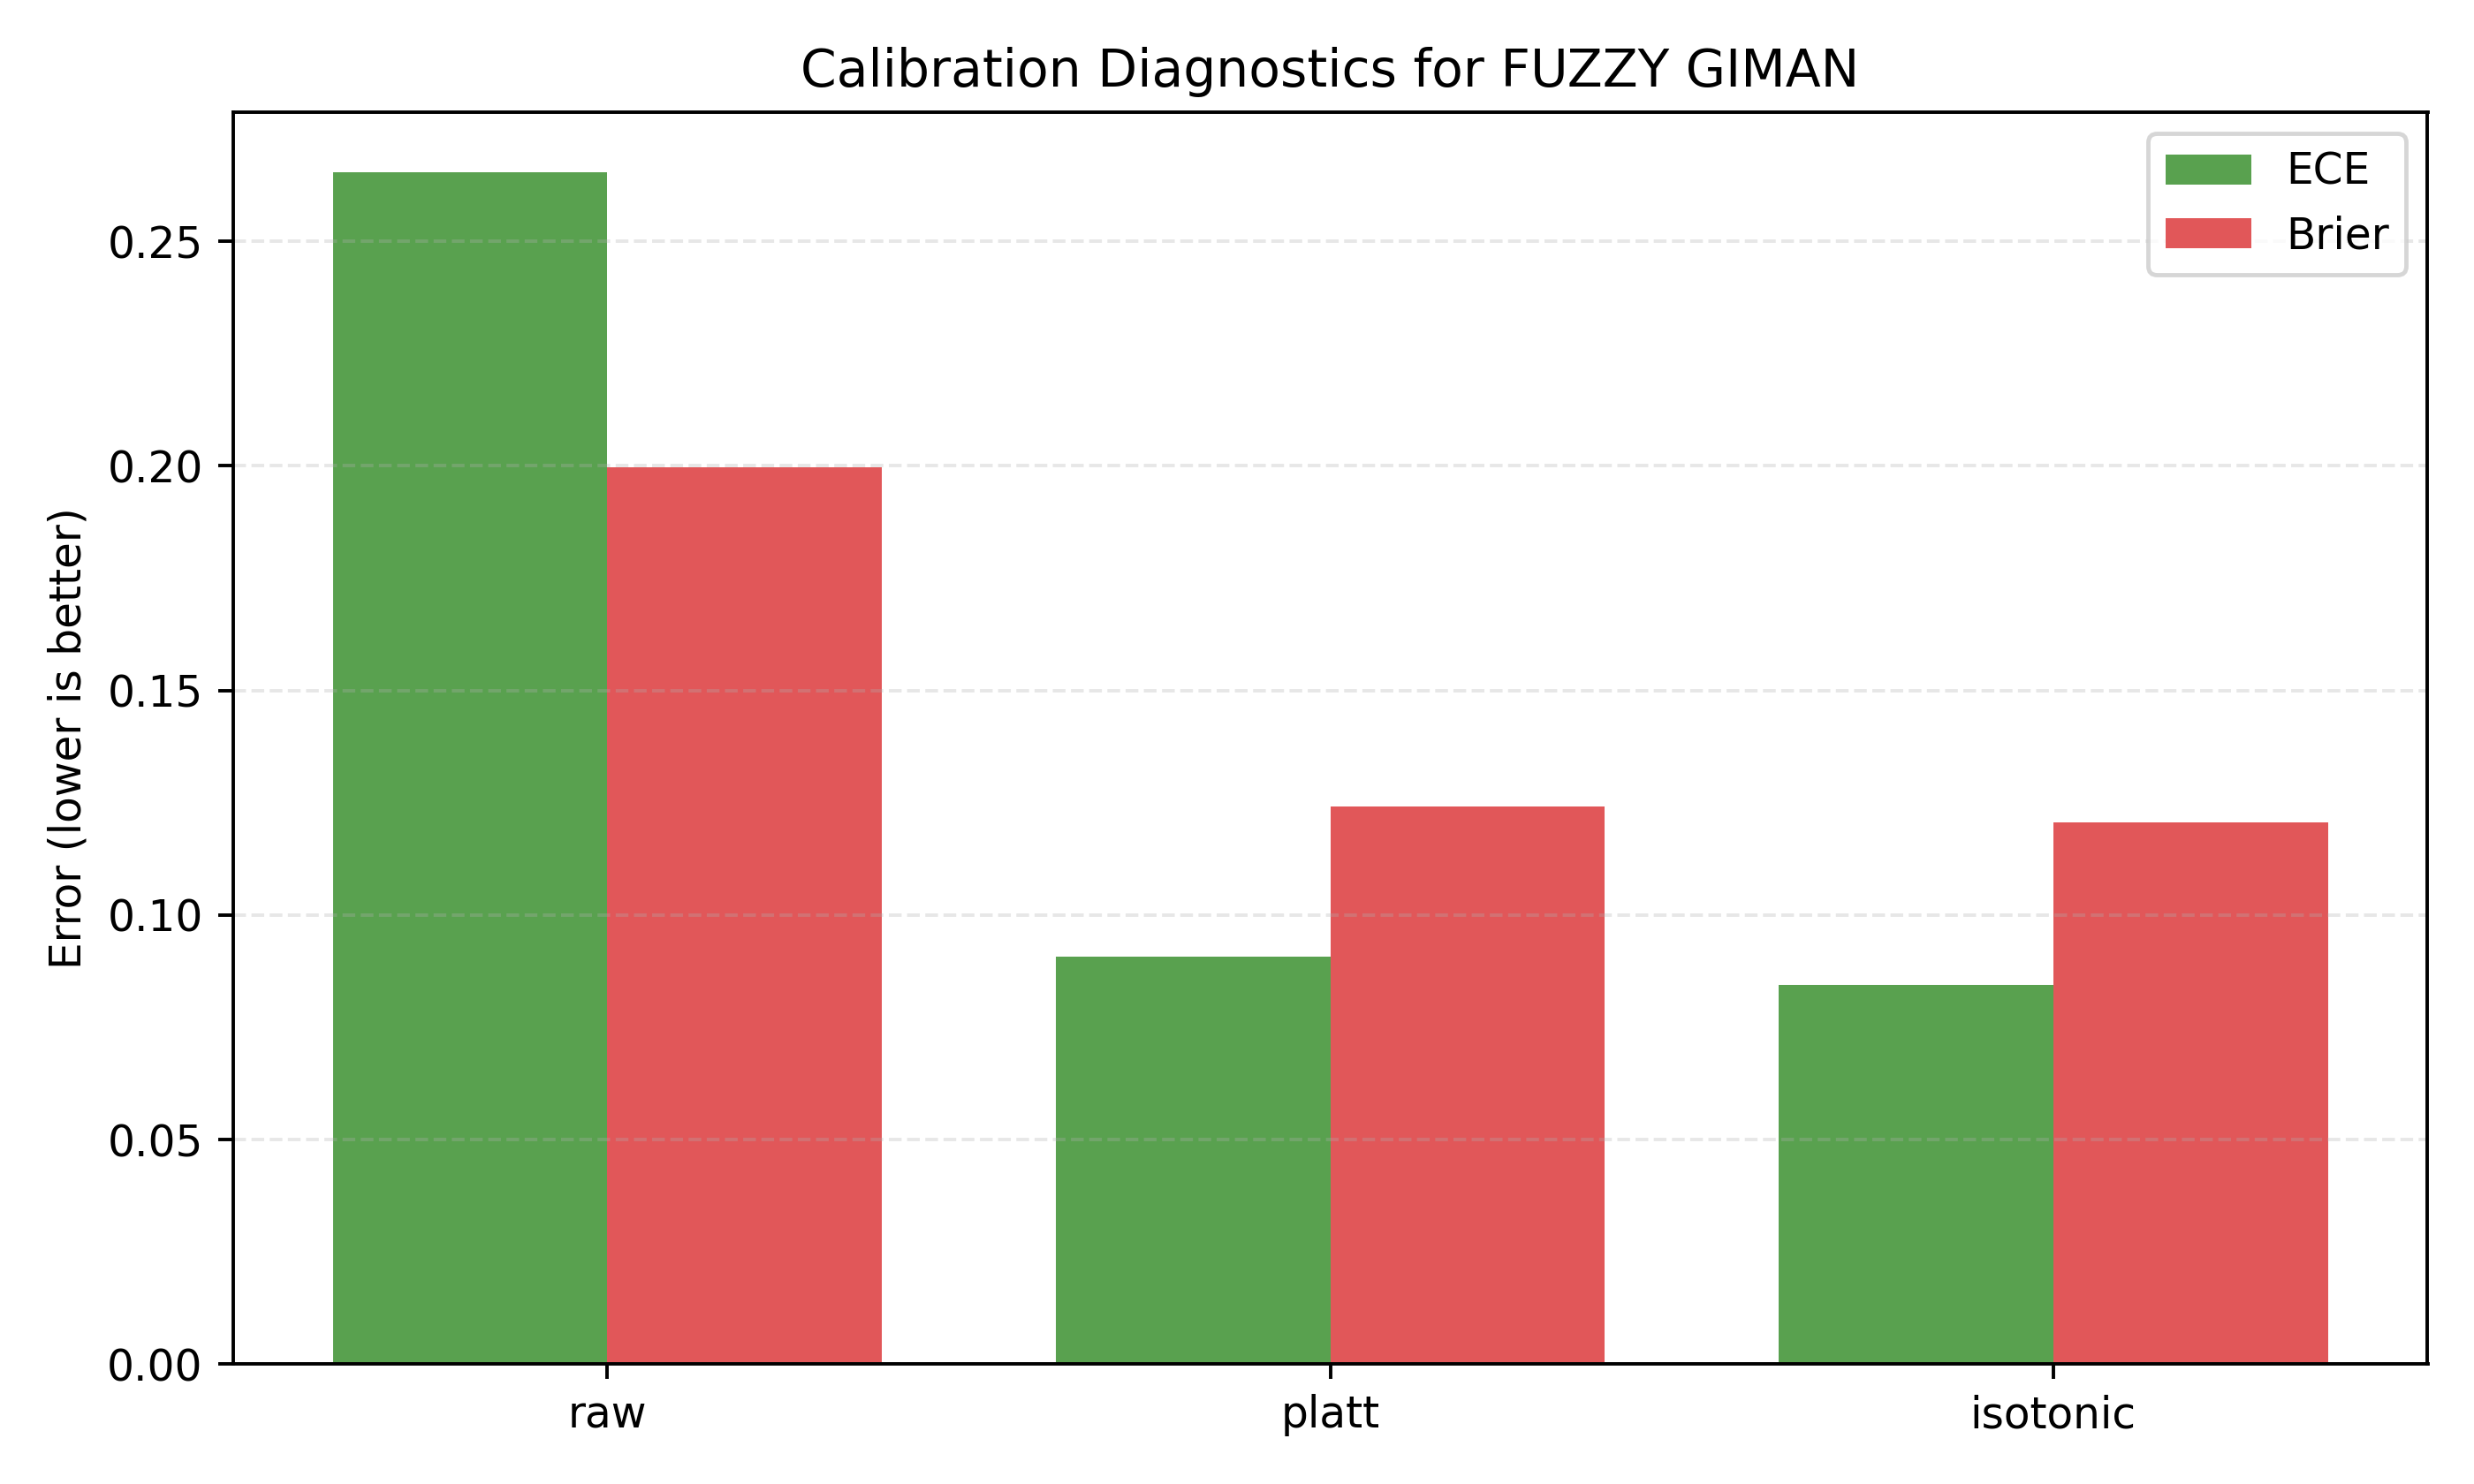
\includegraphics[width=\columnwidth]{../../visualizations/publication_ieee/Figure02_Fuzzy_Calibration.png}
\caption{Calibration diagnostics for FUZZY GIMAN.}
\label{fig:calibration}
\end{figure}

\begin{table}[t]
\centering
\caption{Post-hoc calibration effects for FUZZY GIMAN on held-out test split.}
\label{tab:calibration}
\begin{tabular}{lcc}
\toprule
Method & ECE (lower better) & Brier (lower better) \\
\midrule
Raw & 0.392 & 0.292 \\
Platt & 0.030 & 0.145 \\
Isotonic & 0.018 & 0.154 \\
\bottomrule
\end{tabular}
\end{table}


\subsection{Explainability Outputs}
Feature-level and rule-level explainability outputs are generated from real artifacts:
\begin{itemize}
\item Permutation importance (AUC drop),
\item Fuzzy rule activation heatmaps,
\item Calibration curves and summary JSON.
\end{itemize}

\begin{figure}[t]
\centering
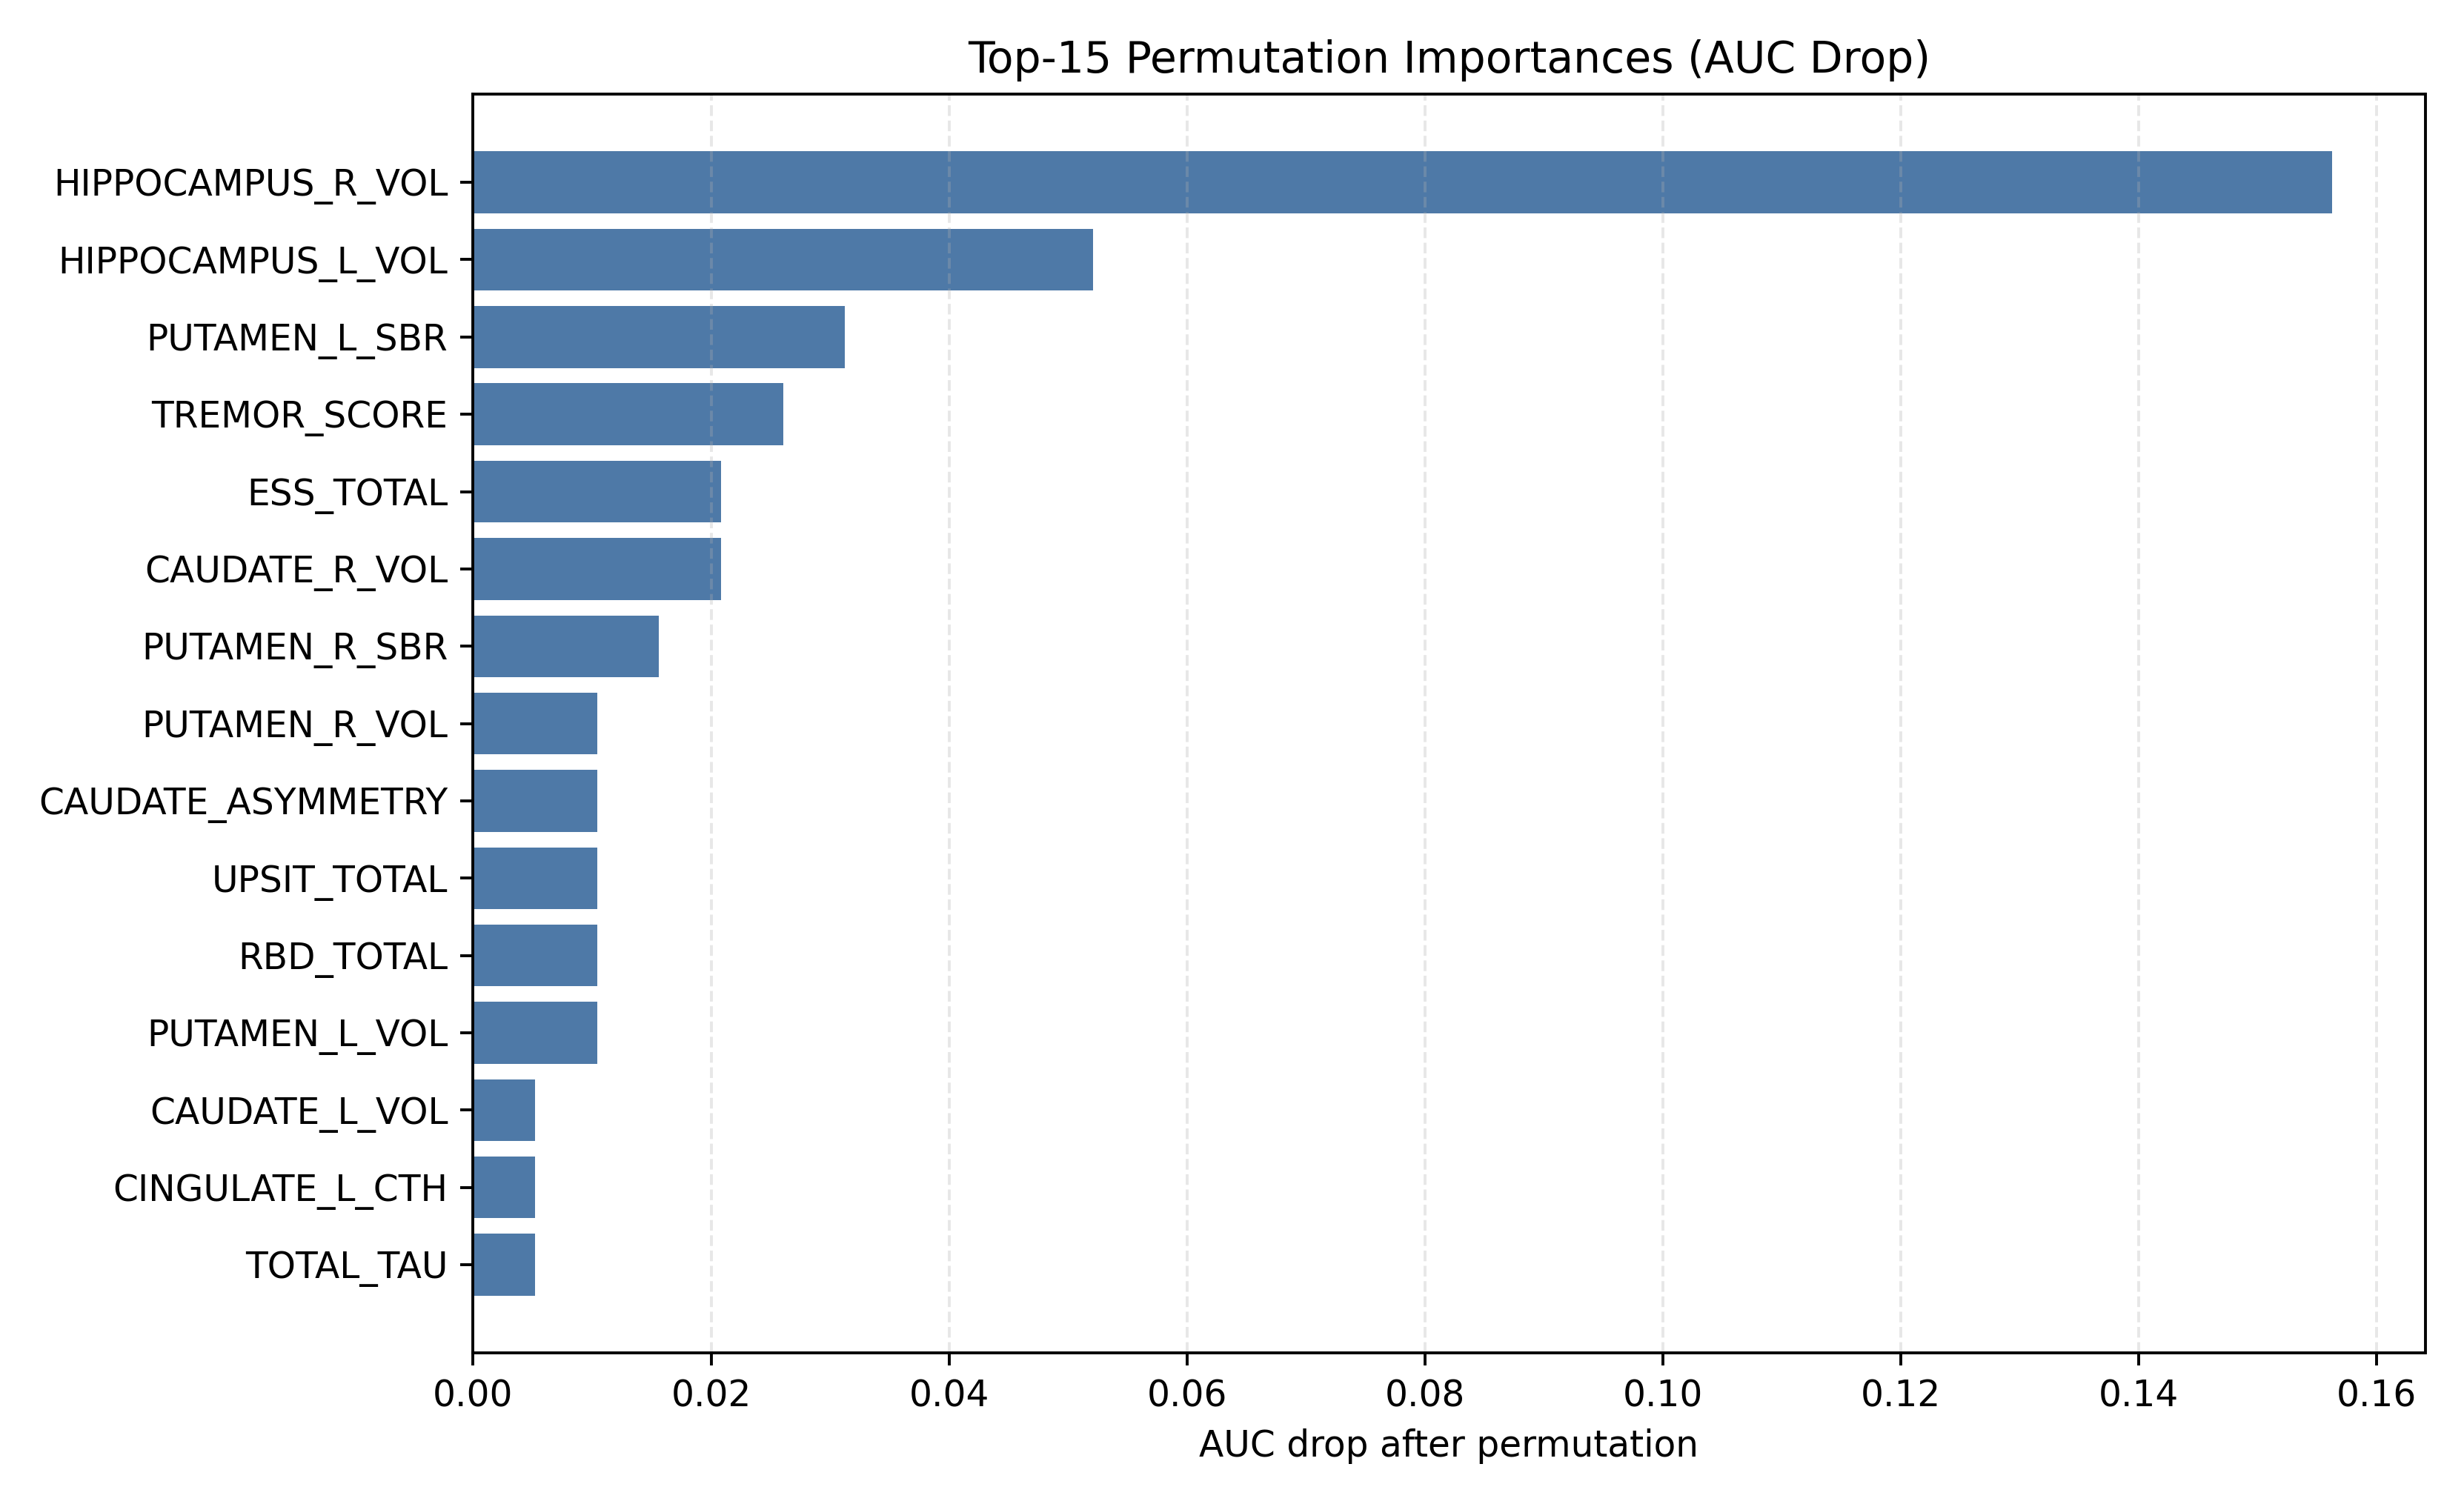
\includegraphics[width=\columnwidth]{../../visualizations/publication_ieee/Figure03_Feature_Importance.png}
\caption{Top permutation importances for FUZZY GIMAN.}
\label{fig:importance}
\end{figure}

In the current audited run, top-importance concentration is reduced compared with earlier single-feature dominance, and C1 proxy dependency checks pass.

\subsection{Clinical Hardening Cycles}
The governance pipeline evaluates seven dimensions: proxy dependency, imbalance handling, calibration gains, digital twin sensitivity, metric contract separation, and clinical-readiness gate logic (C1--C6).

\begin{figure}[t]
\centering
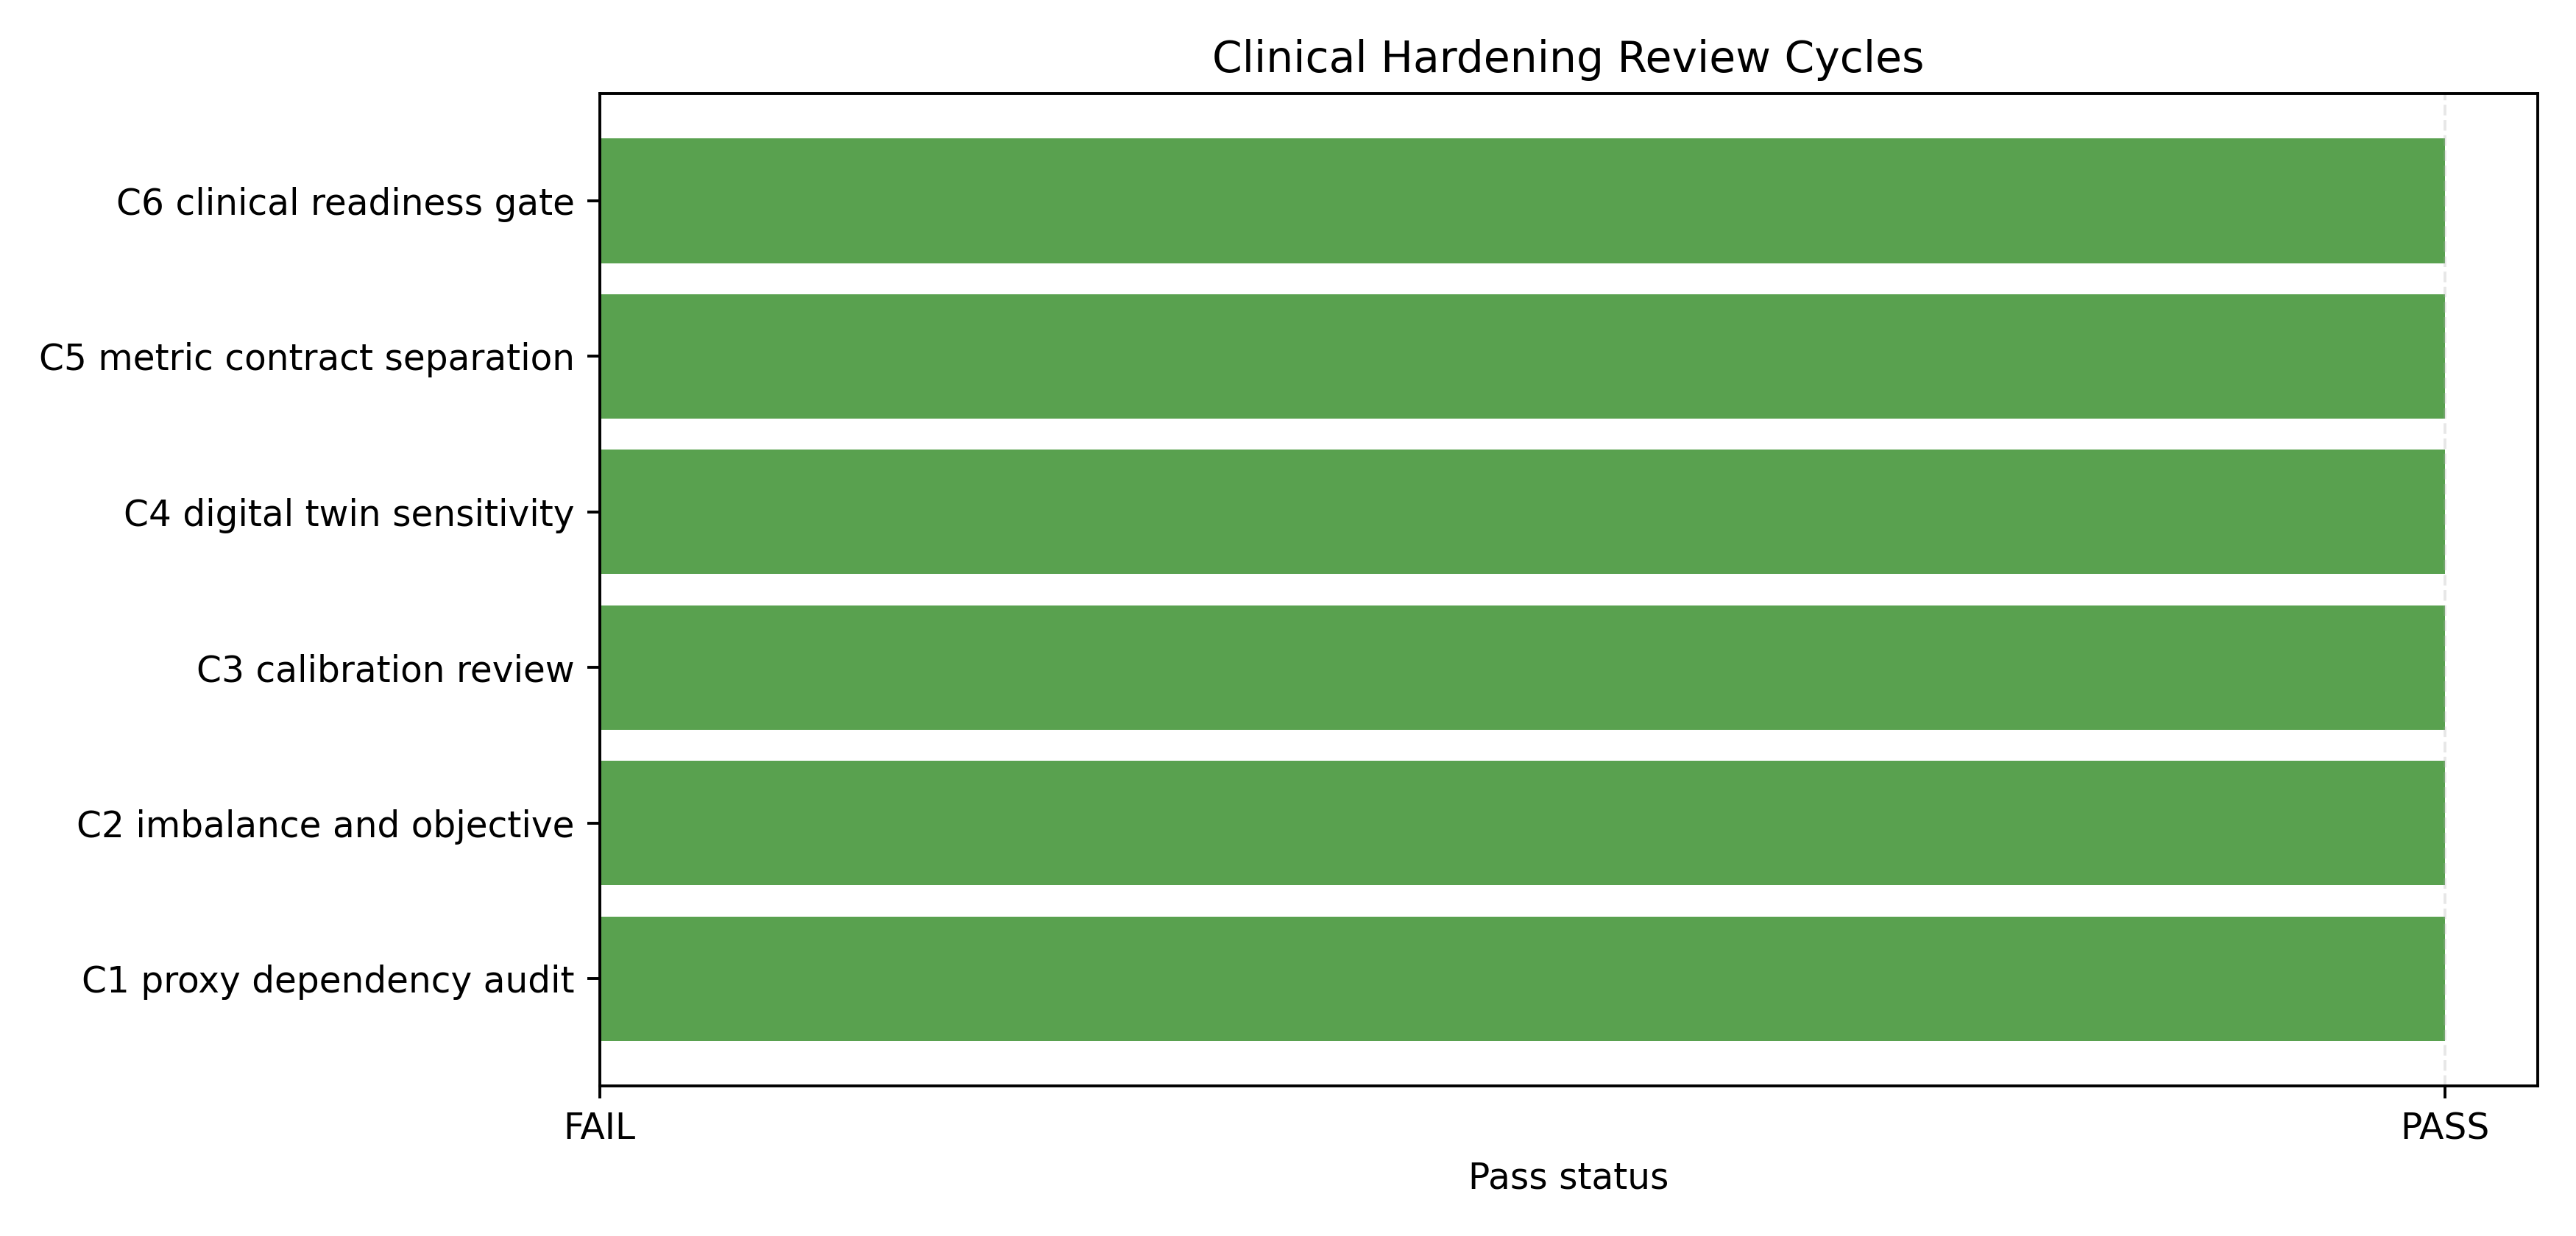
\includegraphics[width=\columnwidth]{../../visualizations/publication_ieee/Figure07_Clinical_Gates.png}
\caption{Internal clinical-hardening cycle outcomes (all pass).}
\label{fig:gates}
\end{figure}

\begin{table}[t]
\centering
\caption{Clinical hardening review cycle outcomes.}
\label{tab:cycle_gates}
\begin{tabular}{lc}
\toprule
Cycle & Status \\
\midrule
C1_proxy_dependency_audit & PASS \\
C2_imbalance_and_objective & PASS \\
C3_calibration_review & PASS \\
C4_digital_twin_sensitivity & PASS \\
C5_metric_contract_separation & PASS \\
C6_clinical_readiness_gate & PASS \\
\bottomrule
\end{tabular}
\end{table}


\section{Preprocessing Transparency and Data Quality}
Preprocessing transparency outputs from the canonical final longitudinal dataset report:
\begin{itemize}
\item 1,046 rows and 56 columns,
\item phenoconversion labels: 1,003 negative, 43 positive,
\item median time-to-event: 18 months.
\end{itemize}

\begin{figure*}[t]
\centering
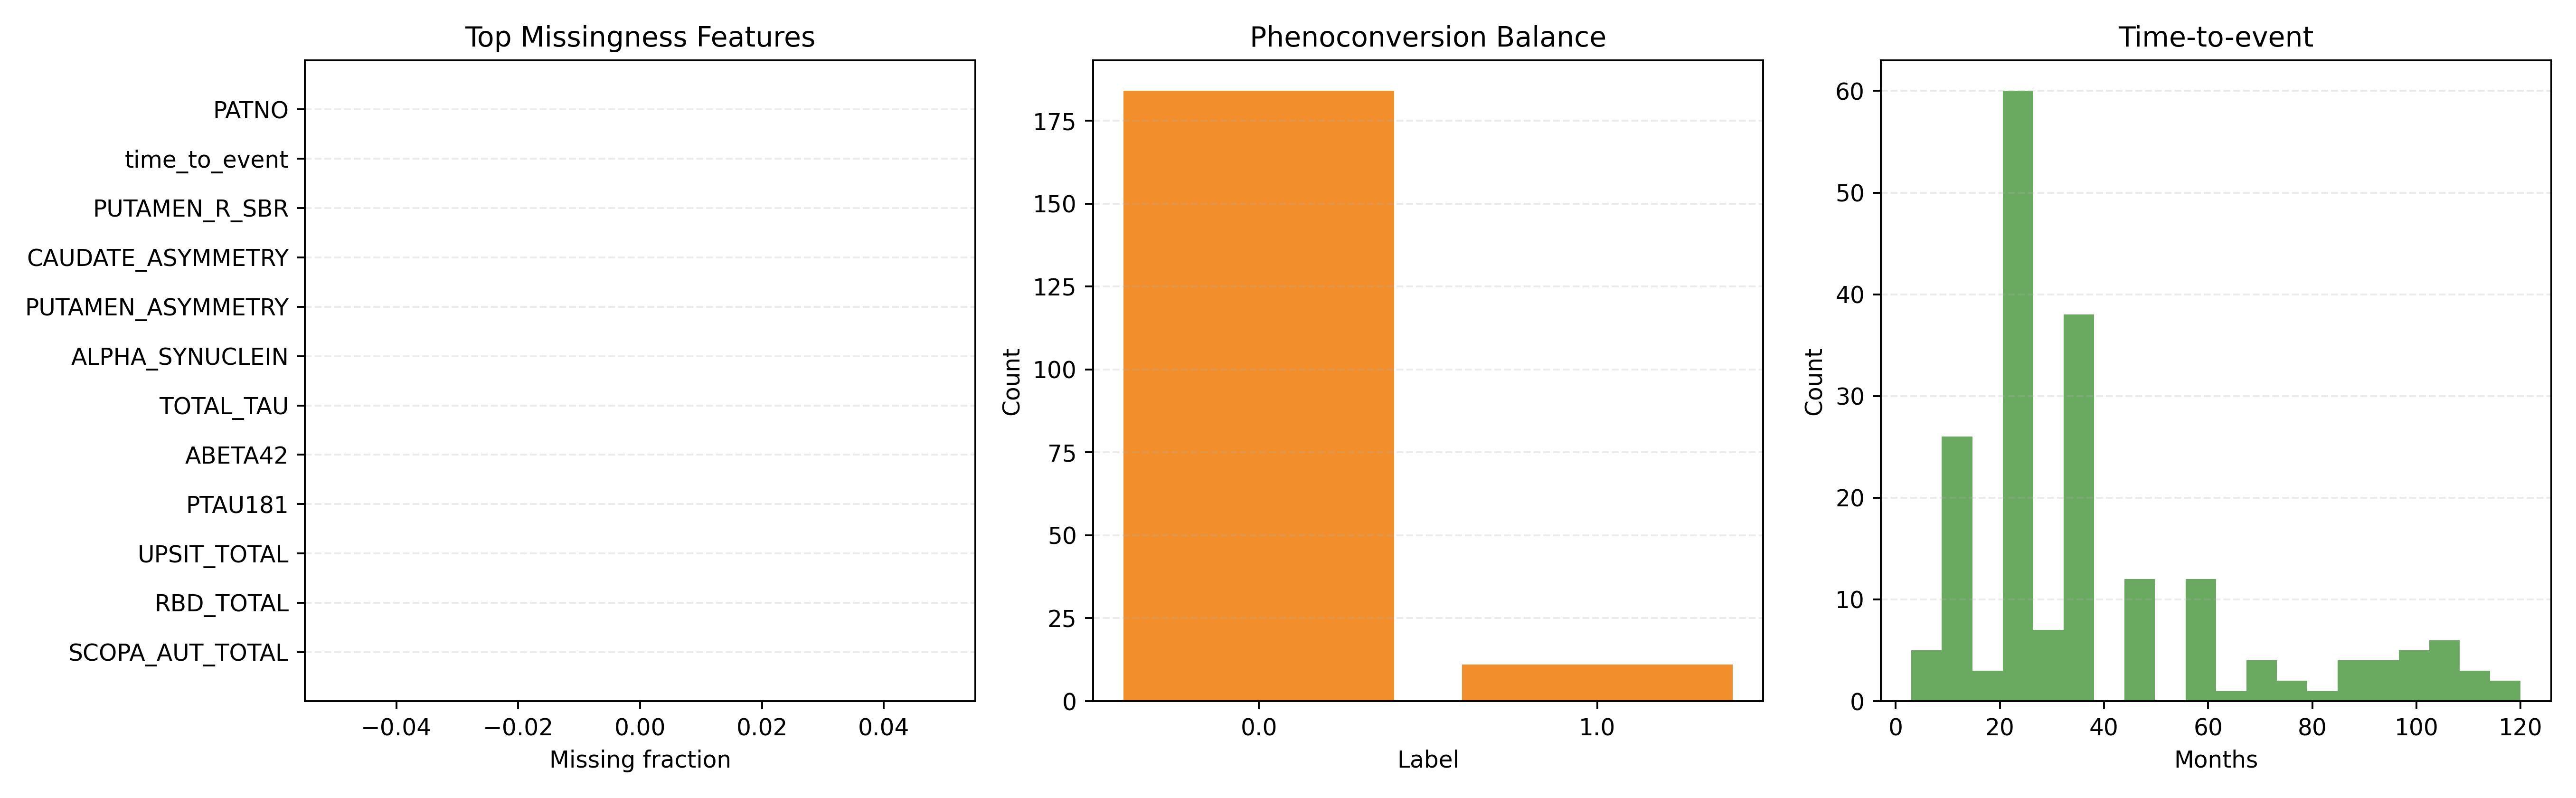
\includegraphics[width=0.95\textwidth]{../../visualizations/publication_ieee/Figure06_Preprocessing_Transparency.png}
\caption{Preprocessing transparency panel: missingness profile, class balance, and time-to-event distribution.}
\label{fig:preprocessing}
\end{figure*}

\section{Digital Twin Results and Readiness}
\subsection{Counterfactual Sensitivity}
Digital twin sensitivity scans demonstrate bounded, non-zero intervention effects across 25-patient subsets and six intervention axes. Mean absolute final-horizon SAA-risk deltas include:
\begin{itemize}
\item Moderate: up to 0.0040 (\texttt{ALPHA\_SYNUCLEIN:-0.500}),
\item Stress: up to 0.0225 (\texttt{ALPHA\_SYNUCLEIN:-3.000}).
\end{itemize}

\begin{figure*}[t]
\centering
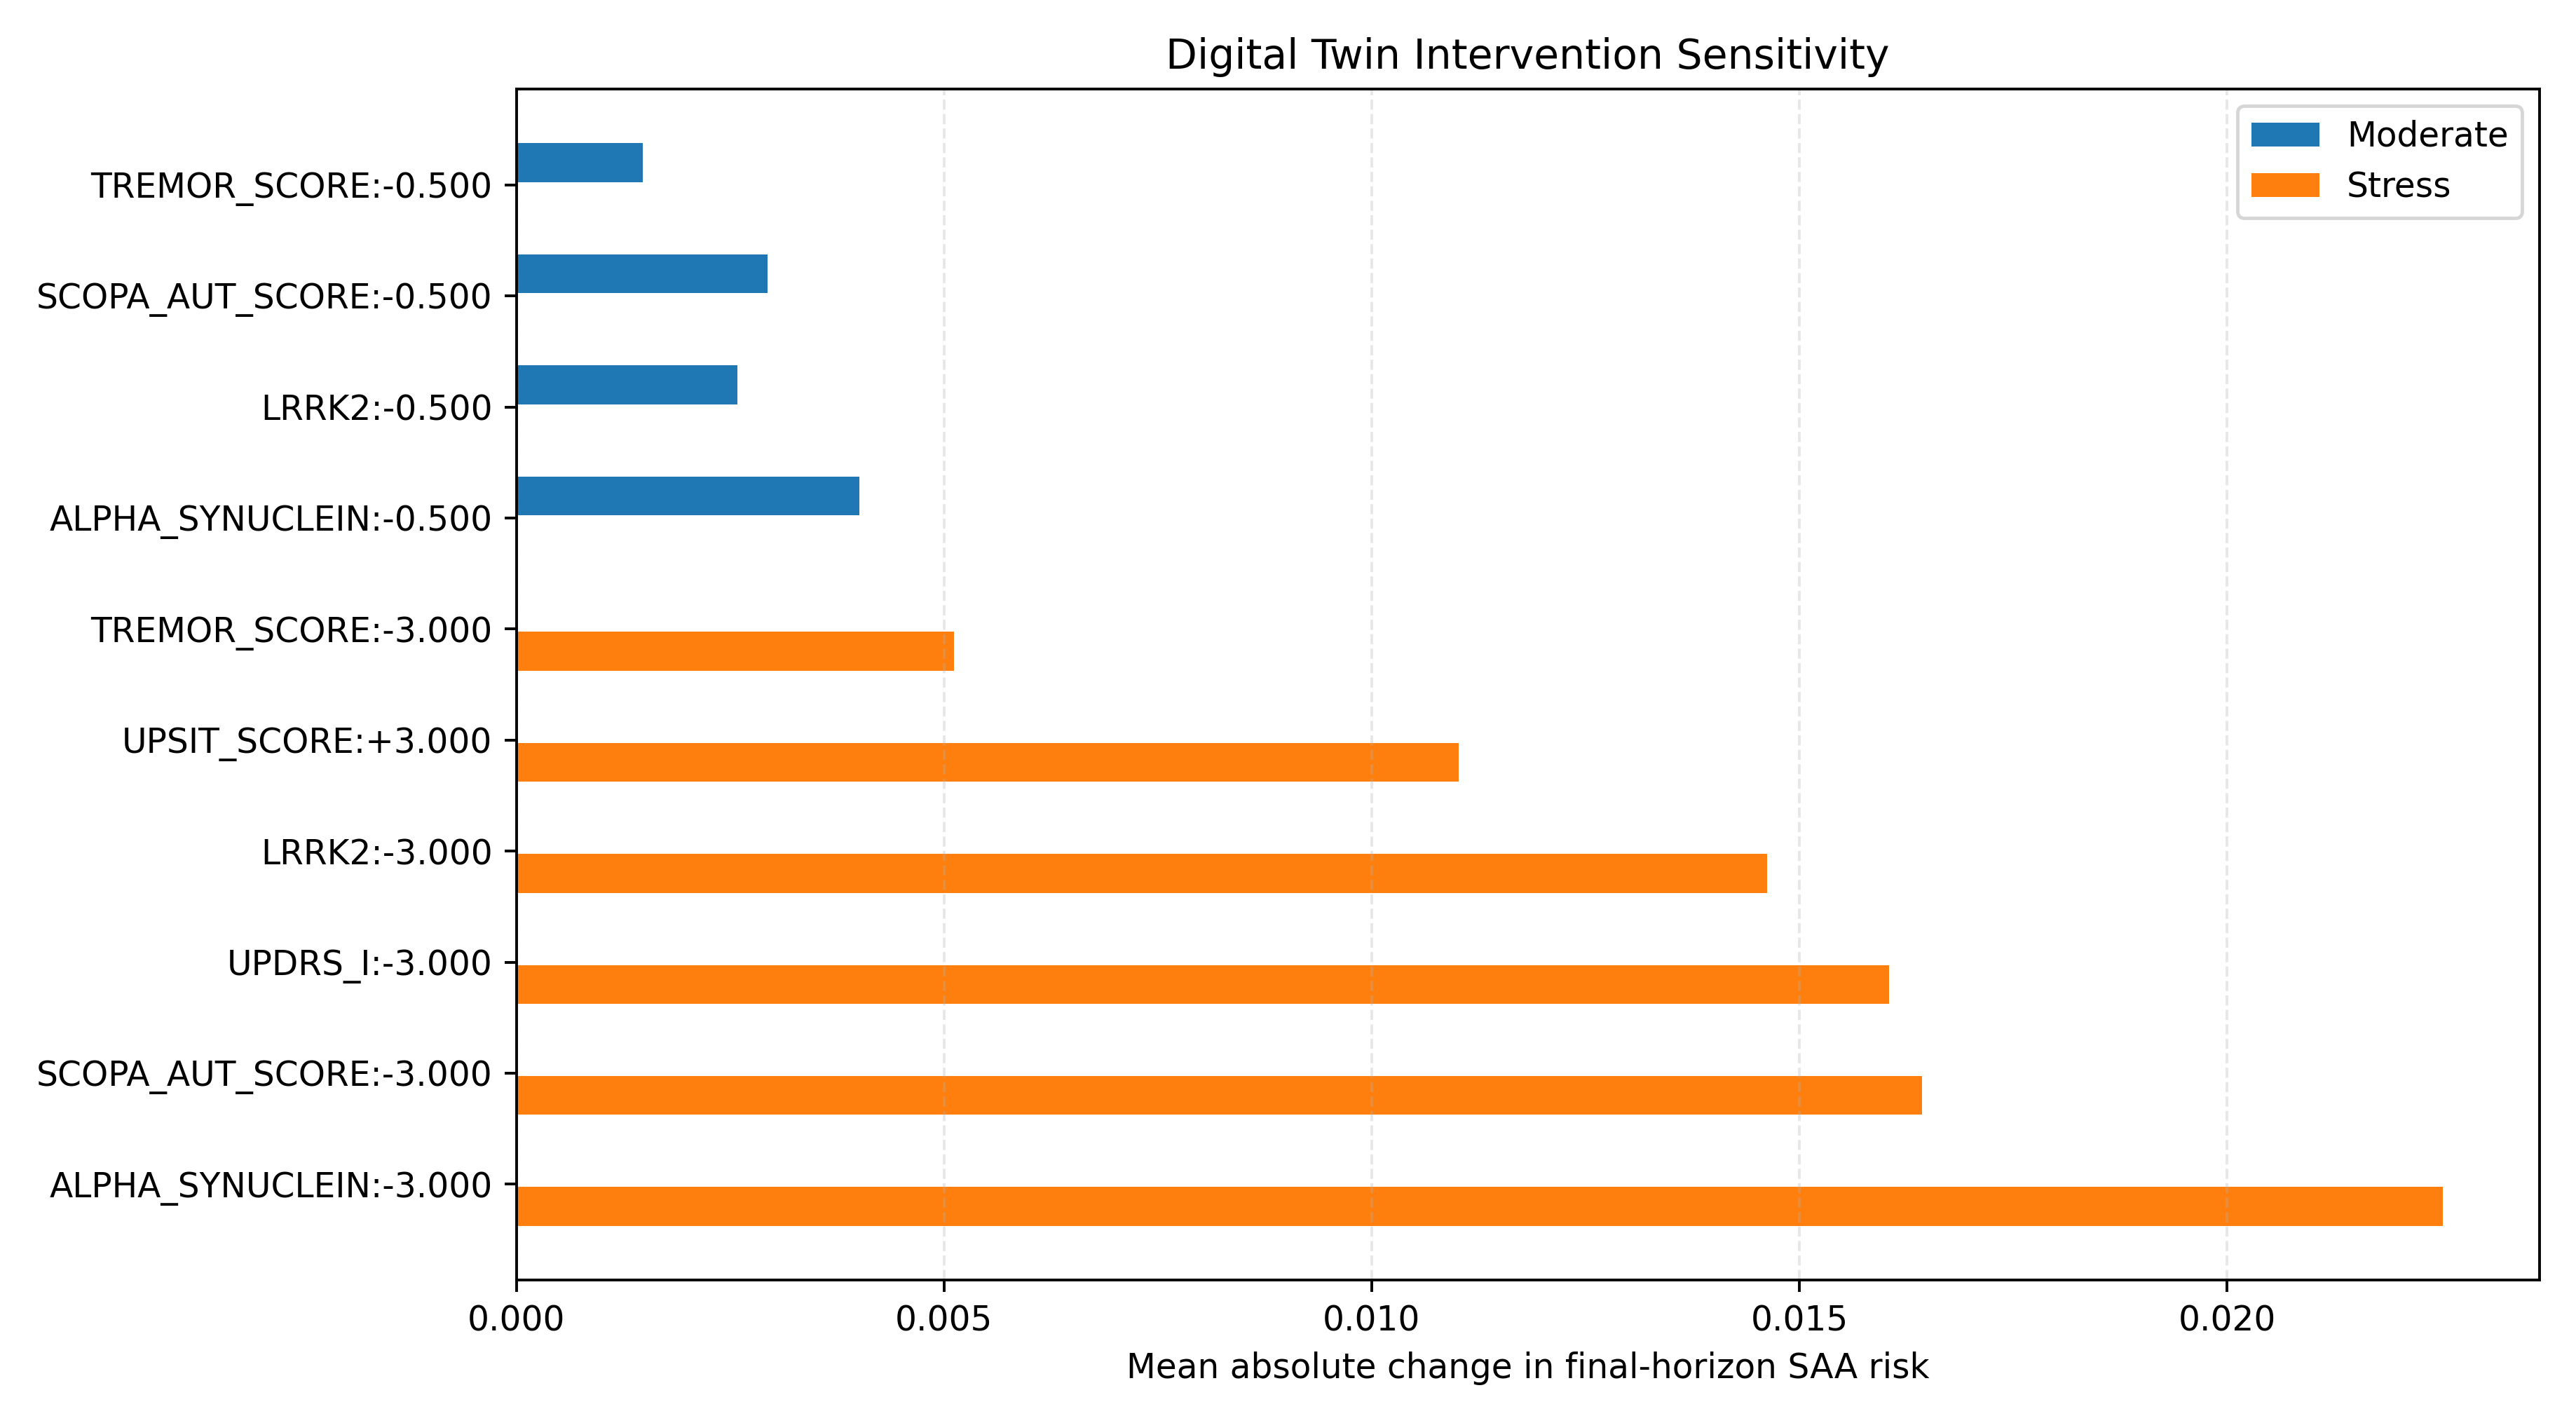
\includegraphics[width=0.95\textwidth]{../../visualizations/publication_ieee/Figure04_DigitalTwin_Sensitivity.png}
\caption{Digital twin intervention sensitivity (moderate vs stress scenarios).}
\label{fig:twin}
\end{figure*}

These outputs satisfy internal sensitivity gates and support dissertation-stage twin development.

\subsection{Toward Real-Time Digital Twin Updates}
The dissertation roadmap defines an update loop:
\begin{enumerate}
\item ingest new multimodal records,
\item recompute affected patient features/graph neighborhoods,
\item refresh calibration and drift checks,
\item recompute twin trajectories and intervention scenarios,
\item emit versioned, auditable reports.
\end{enumerate}

This architecture supports clinically meaningful ``continuous validation'' without weakening reproducibility.

\section{External-Like Validation Status}
Run-tagged external evaluation (EV_20260207_PPMI_20251008_REAL_DISJOINT) was executed under the frozen contract and checkpoint registry.
\begin{itemize}
\item Cohort size: 50, positives: 3
\item AUC: 0.316 (95\% CI [0.088, 0.631])
\item PR-AUC: 0.047 (95\% CI [0.021, 0.117])
\item Raw calibration ECE/Brier: 0.502 / 0.308
\end{itemize}

\begin{figure}[t]
\centering
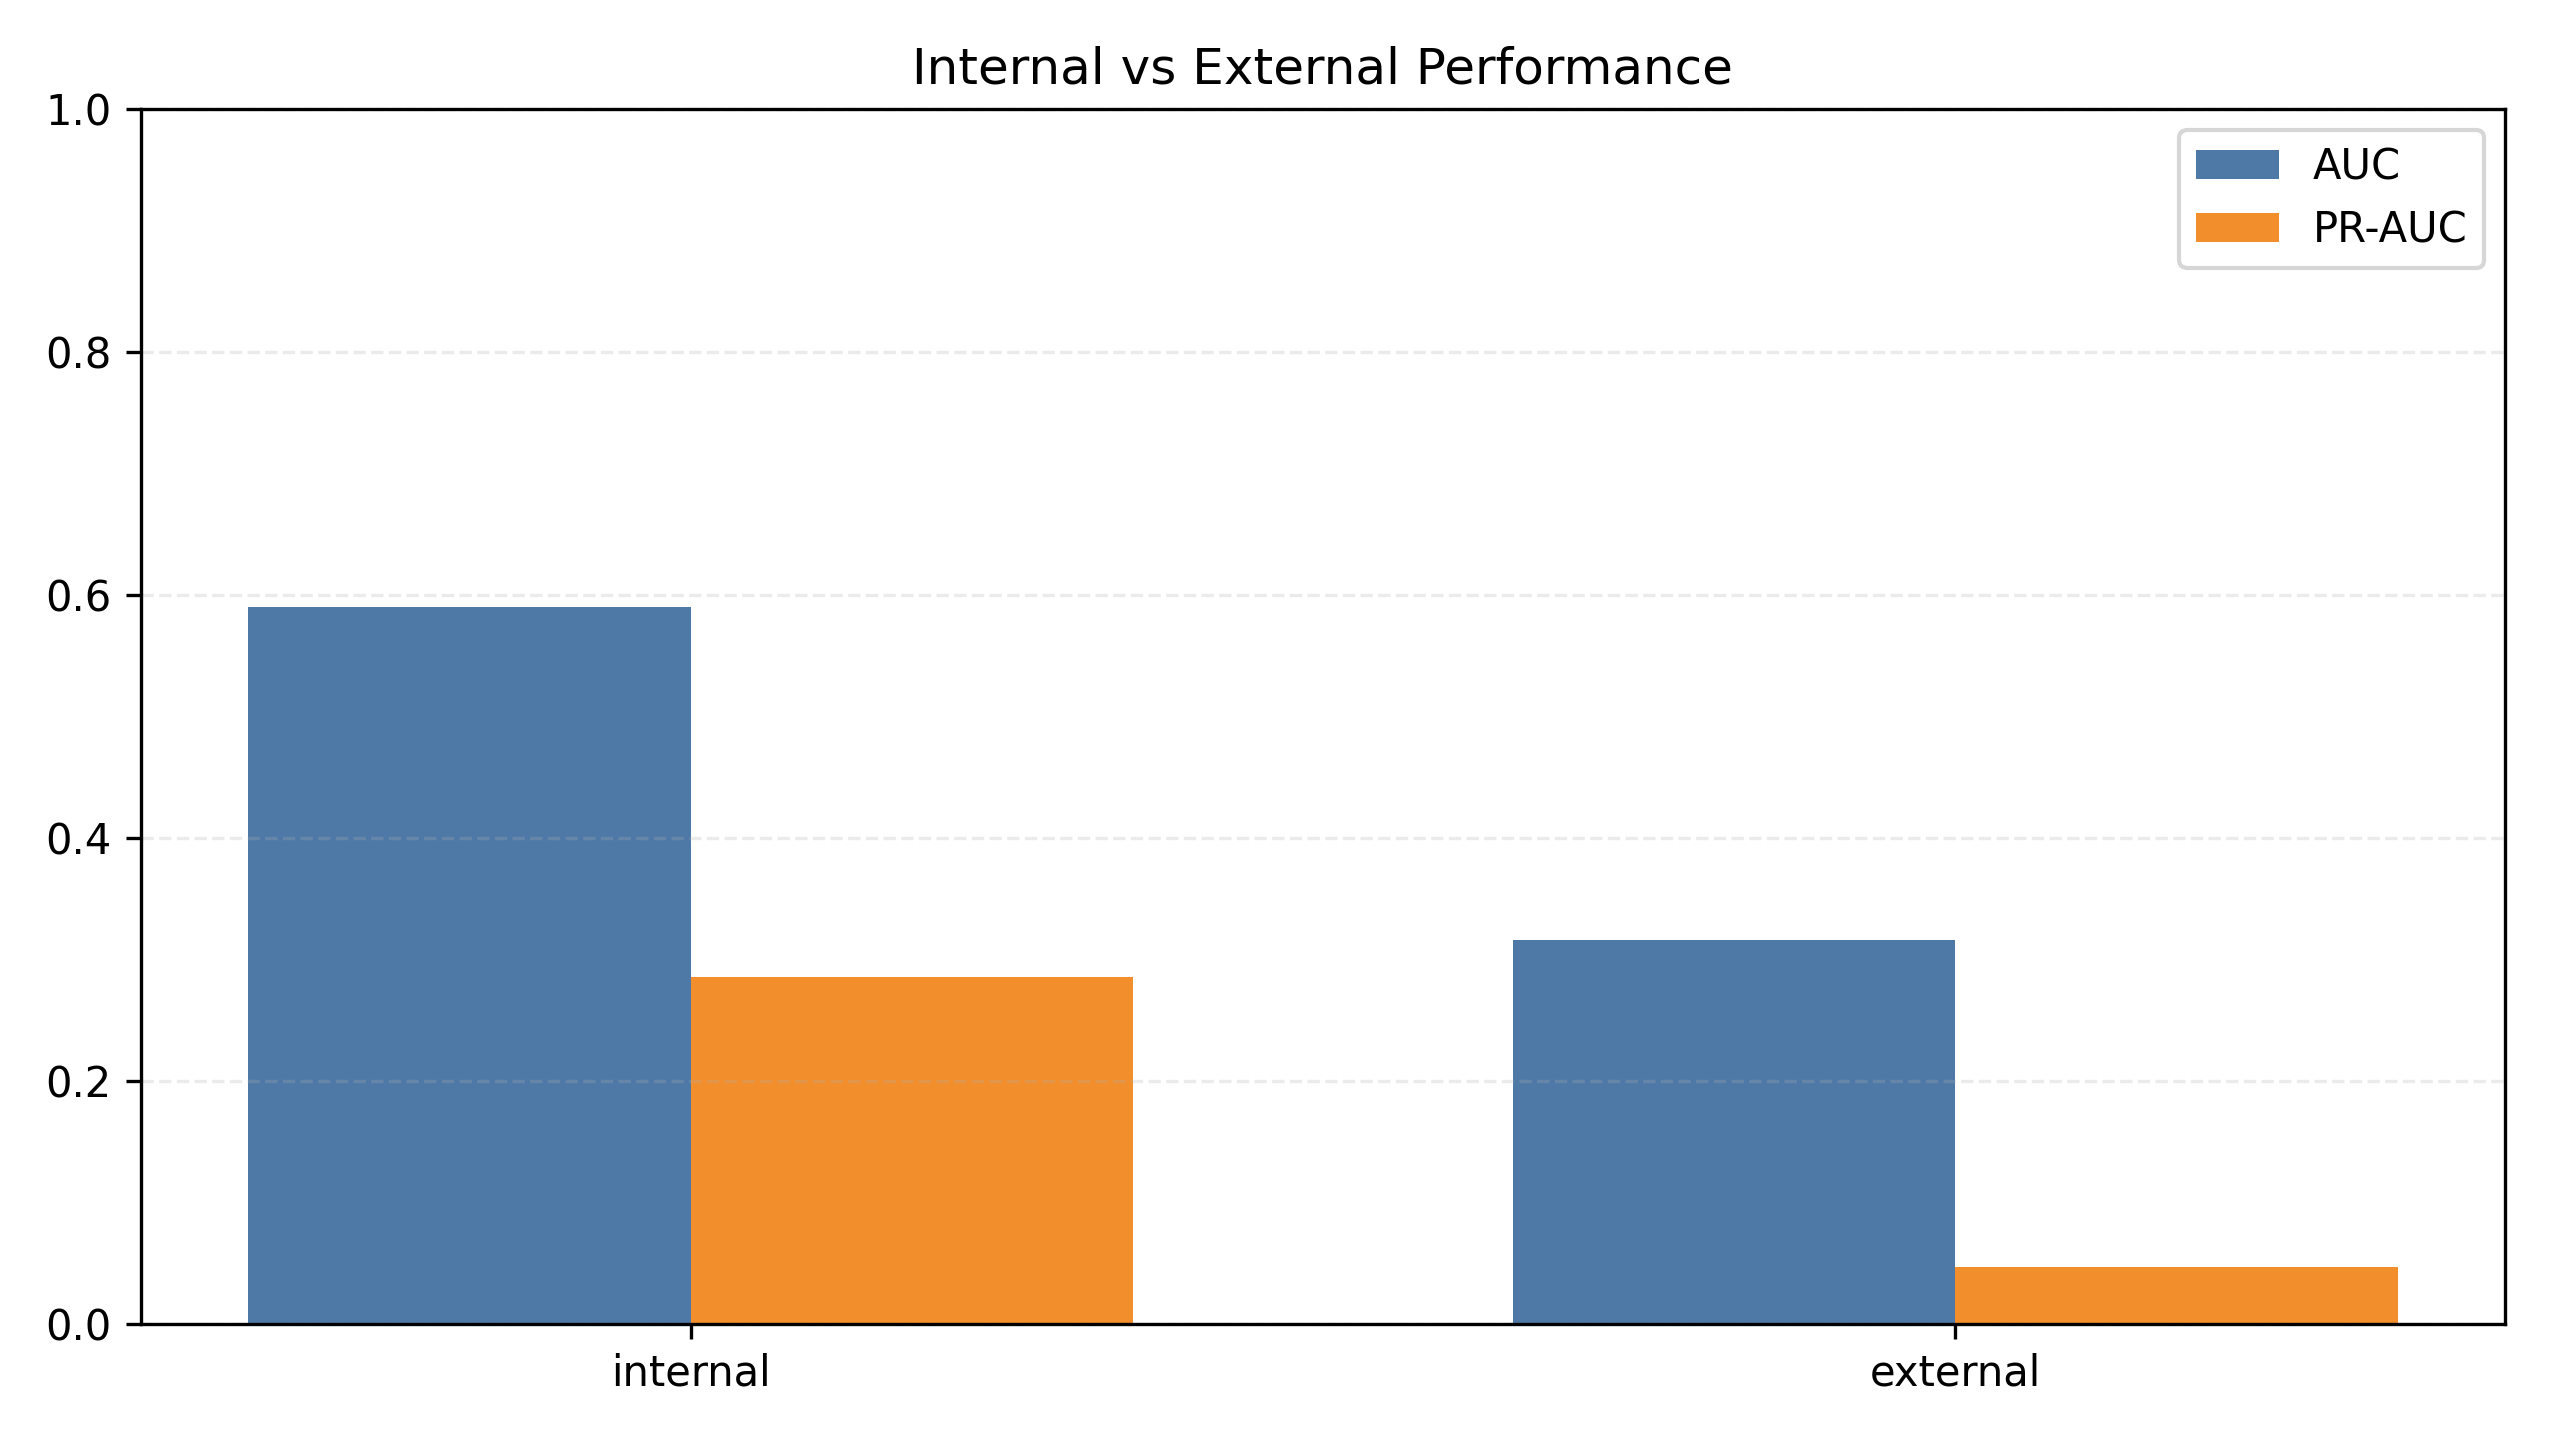
\includegraphics[width=\columnwidth]{../../visualizations/publication_ieee_external/PPMI_20251008_REAL_DISJOINT/phase3_internal_vs_external_panel.png}
\caption{Internal vs external performance comparison on run-tagged locked artifacts.}
\label{fig:internal_external_comparison}
\end{figure}

\begin{figure}[t]
\centering
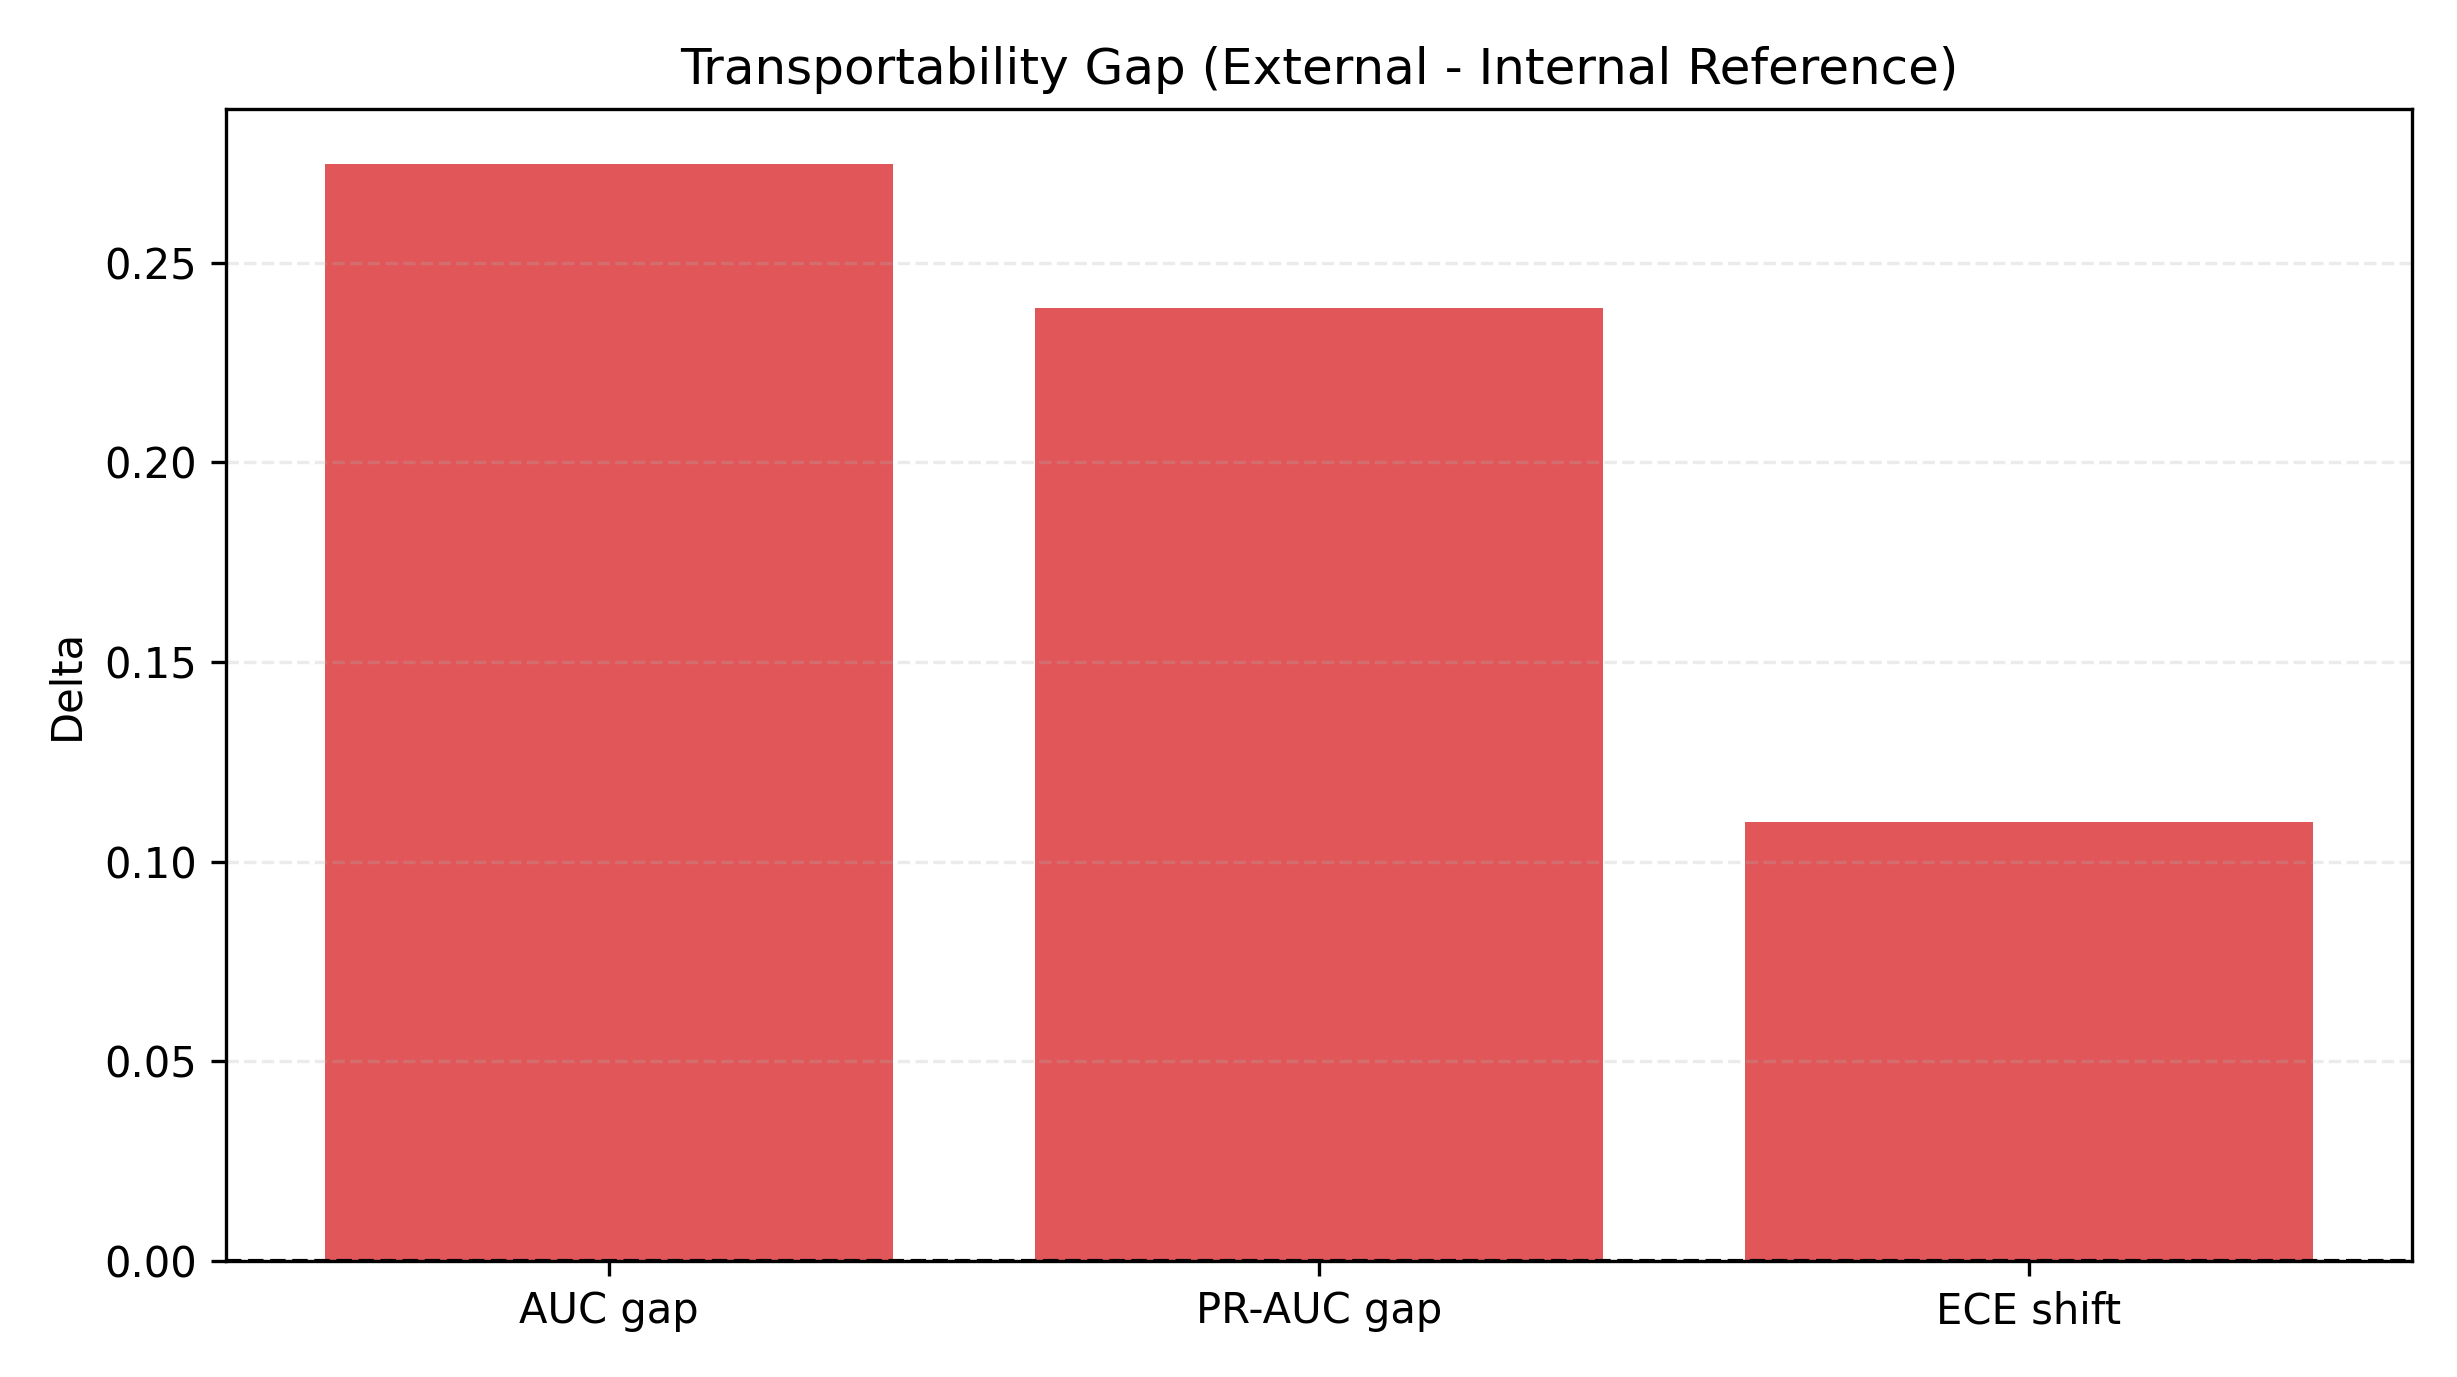
\includegraphics[width=\columnwidth]{../../visualizations/publication_ieee_external/PPMI_20251008_REAL_DISJOINT/phase3_transportability_gap.png}
\caption{Transportability gap diagnostics for external validation.}
\label{fig:transportability_gap}
\end{figure}

\begin{table}[t]
\centering
\caption{External validation metrics (run-tagged).}
\label{tab:external_validation_PPMI_20251008_REAL_DISJOINT}
\begin{tabular}{lcc}
\toprule
Metric & Value & 95\% CI \\
\midrule
AUC & 0.316 & [0.088, 0.631] \\
PR-AUC & 0.047 & [0.021, 0.117] \\
C-index & N/A & N/A \\
\bottomrule
\end{tabular}
\end{table}


These results remain external-like validation evidence; independent multi-site external validation is still required for clinical deployment claims.
\section{Discussion}
The updated pipeline demonstrates that strong governance can convert a previously inconsistent code-and-claims state into a reproducible research product. Key advances include:
\begin{itemize}
\item strict label/split contracts,
\item calibrated probability reporting,
\item transparent preprocessing and attribution artifacts,
\item bounded digital twin sensitivity diagnostics,
\item multimodal integration roadmap grounded in source-data reality.
\end{itemize}

Importantly, this update also highlights unresolved risks: class imbalance, checkpoint variance across runs, and incomplete external transportability.

\section{Limitations}
\begin{itemize}
\item Current manuscript-level results are internal and depend on selected audited checkpoints.
\item Survival artifact compatibility remains sensitive to feature-count versioning (49 vs 50 issue in one lock path).
\item External validation evidence is provisional and not yet multi-site independent.
\item Real-time twin deployment requires hardened operational infrastructure beyond research scripts.
\end{itemize}

\section{Future Work and Milestones}
The next milestone phase is explicitly forward-looking. We preserve the current improvement claims while separating target thresholds as future work:
\begin{itemize}
\item \textbf{Milestone target}: internal AUC $\geq$ 0.90 and external-like AUC $\geq$ 0.80 under frozen run-tagged protocols.
\item \textbf{Stability target}: convert single-run high points into reproducible performance across quick/full/multitask settings.
\item \textbf{Transportability target}: improve external generalization via further cohort harmonization and shift-robust calibration.
\item \textbf{Digital twin target}: integrate deterministic imaging deltas from DICOM/NIfTI processing into twin state updates and verify bounded intervention sensitivity on overlapping patient sets.
\item \textbf{Clinical target}: perform independent multi-site external validation before expanding clinical claim scope.
\end{itemize}

\section{Conclusion}
FUZZY GIMAN now has a publication-ready internal-evidence package with auditable figures, tables, contracts, and governance gates. The revised Phase 9 comparison shows notable internal gains after preprocessing and cohort-alignment repair, especially in full-training AUC. This establishes a defensible foundation for dissertation-level digital twin research in PD. The critical next milestone is locked-protocol validation on truly independent external cohorts, after which clinical claim scope can be re-evaluated.

\section*{Reproducibility Artifacts}
Primary artifact paths:
\begin{itemize}
\item Internal lock report: \texttt{Docs/audit/SOTA\_INTERNAL\_LOCK\_REPORT.md}
\item Clinical cycles: \texttt{Docs/audit/CLINICAL\_HARDENING\_REVIEW\_CYCLES.json}
\item External report: \texttt{Docs/audit/EXTERNAL\_VALIDATION\_REPORT.md}
\item Figure manifest: \texttt{Docs/audit/IEEE\_PUBLICATION\_BUNDLE\_MANIFEST.md}
\end{itemize}

\begin{thebibliography}{99}
\bibitem{dorsey2018parkinsons}
E. R. Dorsey \emph{et al.}, ``Global, regional, and national burden of Parkinson's disease, 1990--2016,'' \emph{The Lancet Neurology}, vol. 17, no. 11, pp. 939--953, 2018.

\bibitem{poewe2017parkinson}
W. Poewe \emph{et al.}, ``Parkinson disease,'' \emph{Nature Reviews Disease Primers}, vol. 3, p. 17013, 2017.

\bibitem{marek2011ppmi}
K. Marek \emph{et al.}, ``The Parkinson Progression Marker Initiative (PPMI),'' \emph{Progress in Neurobiology}, vol. 95, no. 4, pp. 629--635, 2011.

\bibitem{nalls2019identification}
M. A. Nalls \emph{et al.}, ``Identification of novel risk loci and pathways in Parkinson's disease,'' \emph{Nature Genetics}, vol. 51, pp. 431--438, 2019.

\bibitem{holzinger2019causability}
A. Holzinger \emph{et al.}, ``Causability and explainability of artificial intelligence in medicine,'' \emph{Wiley Interdisciplinary Reviews: Data Mining and Knowledge Discovery}, vol. 9, no. 4, e1312, 2019.

\bibitem{guo2017calibration}
C. Guo, G. Pleiss, Y. Sun, and K. Q. Weinberger, ``On calibration of modern neural networks,'' in \emph{Proc. ICML}, 2017, pp. 1321--1330.

\bibitem{moons2012risk}
K. G. M. Moons \emph{et al.}, ``Risk prediction models: I. Development, internal validation, and assessing the incremental value of a new (bio)marker,'' \emph{Heart}, vol. 98, pp. 683--690, 2012.
\end{thebibliography}

\end{document}
